\chapter{EMC Effect}	
\section{European Muon Collaboration}\label{sec:EMC}
\paragraph{}The European Muon Collaboration (EMC) performed a deep inelastic measurement with 120-280 GeV muons on iron, hydrogen, and deuteron targets to begin a comprehensive study of ,muon scattering \cite{challenge, Norton}. The EMC used muons in order to reach their goal of achieving interactions at a large $Q^2$ \cite{seelyth}. The EMC studied the per nucleon normalized Fe/D structure function ratio versus the Bjorken scaling variable, $x$. The EMC expectations for this ratio originally was unity for $x$ between 0.05 and 0.7 and would deviate at higher $x$ due to Fermi smearing\cite{CC}. The reasoning for this expectation was the belief that at large magnitude of $Q^2$ the interaction between protons and neutrons would not contribute to the total structure function of the nucleus. This was the understanding because the binding energy of a few MeV would not interferer with the GeV scale of the DIS interaction \cite{Ajth}. The expected structure function for a nucleus could be written as:
\begin{equation}
F_2^A = N F_2^N + ZF_2^P.
\end{equation}
In this quasi-free nucleon picture, the nucleons are used to build up the nuclear structure ($F_2^A$) by summing up the neutron structure function ($F_2^N$) with the proton structure function($F_2^P$) for each nucleon. Their results for their ration comparison of iron and deuterium are shown in Figure \ref{EMCOld}. The $\frac{A}{D}$ structure function ratio showed an unexpected downward slope. This phenomenon was titled the EMC effect. This finding demonstrated to the EMC that their understanding of the nucleus was incorrect. A nucleon's structure function and thereby, the constituent quark distributions are altered by the structure of the nuclear medium. 
\begin{figure}[h]
	\centering
	\caption{ Graph of the ratio of A/D structure functions vs $x$ from the EMC. \cite{CC,EM}.}
	\label{EMCOld}
	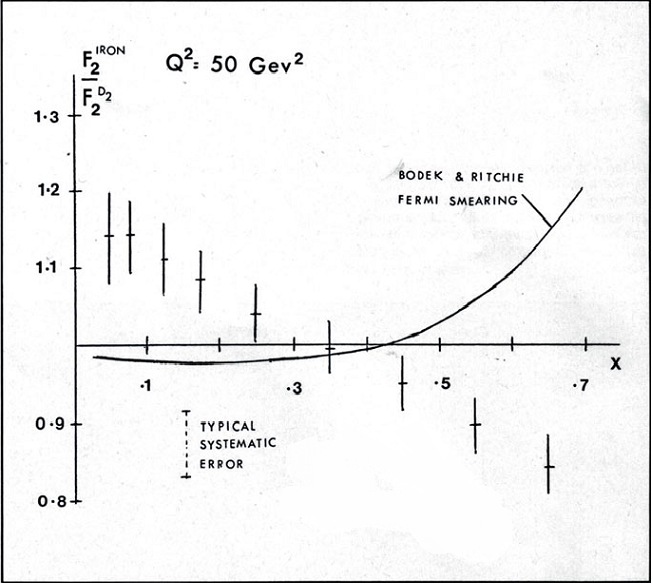
\includegraphics[width=10cm]{EMC.png} 
\end{figure} 
\section{Ratios - Cross Sections and Structure Functions}
\paragraph{}In chapter one we defined the  inelastic cross section in equation \ref{ISCS}.  
\begin{equation}
\label{ISCSch2}
\sigma^A=\frac{4\alpha^2E^{\prime 2}}{Q^4} \bigg\lbrack 2\frac{F_1^A(x)}{M}sin^2\frac{\theta}{2} + \frac{F_2^A(x)}{\nu}cos^2\frac{\theta}{2} \bigg \rbrack.
\end{equation} 
In figure \ref{EMCOld}, the EMC collaboration analyze the ratio of $F_2$ structure functions. The per nucleon cross section of two different nuclei can be reduced to ratio of the $F_2$ structure functions.  
\begin{equation}
\label{rat}
\frac{\sigma_{A_2}}{\sigma_{A_1}} = \frac{F_2^{A_2}}{F_2^{A_1}}
\end{equation}
The reduction of the ratio of two nuclei begin by using the ratio of longitudinal and transverse cross sections as a function of $F_1/F_2$.
\begin{equation}
R=\frac{\sigma_{L}}{\sigma_{T}} =\left(1+\frac{\nu^2}{Q^2} \right)\frac{MF_2}{\nu F_1} -1
\label{Rratio}
\end{equation}
The ratio of two unique per nucleon cross sections is:
\begin{equation}
\label{Aratio}
\frac{\sigma_{A_2}}{\sigma_{A_1}} = \frac{F_2^{A_2}}{F_2^{A_1}} \frac{\left[1+ 2\frac{\nu F_1^{A_2} }{MF_2^{A_2}} tan^2\frac{\theta}{2} \right]}{\left[1+ 2\frac{\nu F_1^{A_1} }{MF_2^{A_1}} tan^2\frac{\theta}{2} \right]}
\end{equation}
Where $A_1$ and $A_2$ denote the different nuclei. Using the definition of $R$ in equation \ref{Aratio}, the per nucleon cross section ratio of $A_1$ and $A_2$ can be simplified to equation \ref{rat} \cite{EM,seelyth}. The simplification of the cross section ratio to the structure function ratio is based on the use of $R$. The longitudinal and transverse cross section ratio has been study extensively for many nuclei. The measurements of $R$ have shown no dependence on the number of nucleons \cite{EM}. 
\paragraph{}The $x$ spectrum of a per nucleon cross section ratio of some nucleus with A nucleons and deuterium also known as an $A/D$ ratio or an EMC ratio is broke into 4 different regions. 
\begin{itemize}
	\item For $x < 0.1$, the shadowing region has an EMC ratio that shows a decline of the nuclear stricture functions. A coupling of the photon to strongly interacting quarks causes this feature \cite{PnN}.
	\item The anti-shadowing region of the $x$ spectrum lies at $0.1 \leq x < 0.3 $. The results of DIS experiments show an EMC ratio slightly larger then unity in this region. This increase is caused by constructive interference among the multi-scattering amplitudes in the nucleus \cite{shadowing}.
	\item $X$ between 0.3 and 0.7 is the EMC effect region. This region will be discussed furtherer in this chapter.
	\item For $X > 0.7$, the EMC ratio grows rapidly above unity.  This region is the Fermi-motion region. The  motion of the nucleons inside a nucleus creates distribution of the nucleons'  momentum. The convolution between the nucleons' structure function and momentum distribution form the nuclear structure function. This causes nuclear structure function of an A $> 2$ nucleus to rise quickly compared to a deuterium nucleus \cite{Ajth,PnN}. 
\end{itemize}
\section{EMC Experiments}
\subsection{Experiments at CERN}
\paragraph{EMC} The EMC published results from muon beam experiments in 1981-1983 \cite{EMC_iron,EM,EMC_F2d,CERN_EMC}.  The EMC used data from this group of experiments to form the first EMC ratios, shown in \ref{EMCOld}. The experiments used muon beams of 120 to 280 GeV to extract nuclear and nucleon structure functions from iron, deuterium and Hydrogen targets. The use of multiple indecent beam energies allowed these experiments to have a $Q^2$ for $x$ of 0.05 between 8 and 20 GeV$^2$ and a $Q^2$ for $x$ of 0.65 between 35 and 200 GeV$^2$ \cite{CERN_EMC}. Through out the this run of experiments the EMC used the EMC forward detector but the experiments were conducted at different times causing a rise in the total uncertainties for the EMC ratios\cite{EM}. After publishing the results for the EMC effect, the EMC conducted another round of experiments for two reasons. First the EMC focused on decreasing the systematic uncertainties that were seen in the first EMC effect analysis. They also want to expand the knowledge of the EMC effect of more nuclei \cite{EMC_ext, Ajth}. This included measuring muon scattering on carbon, copper, and tin \cite{EMC_ext}.

\begin{figure}[H]
	\caption{EMC effect from the BCDMS collaboration \cite{BCDMS}. The BCDMS results show in plot 'a' a good comparison from their EMC effect for iron and the results from the EMC. In plot 'b', BCDMS collaboration compare their nitrogen EMC results to SLAC's carbon EMC results.}
	\label{fig:BCDMS}
	\centering
	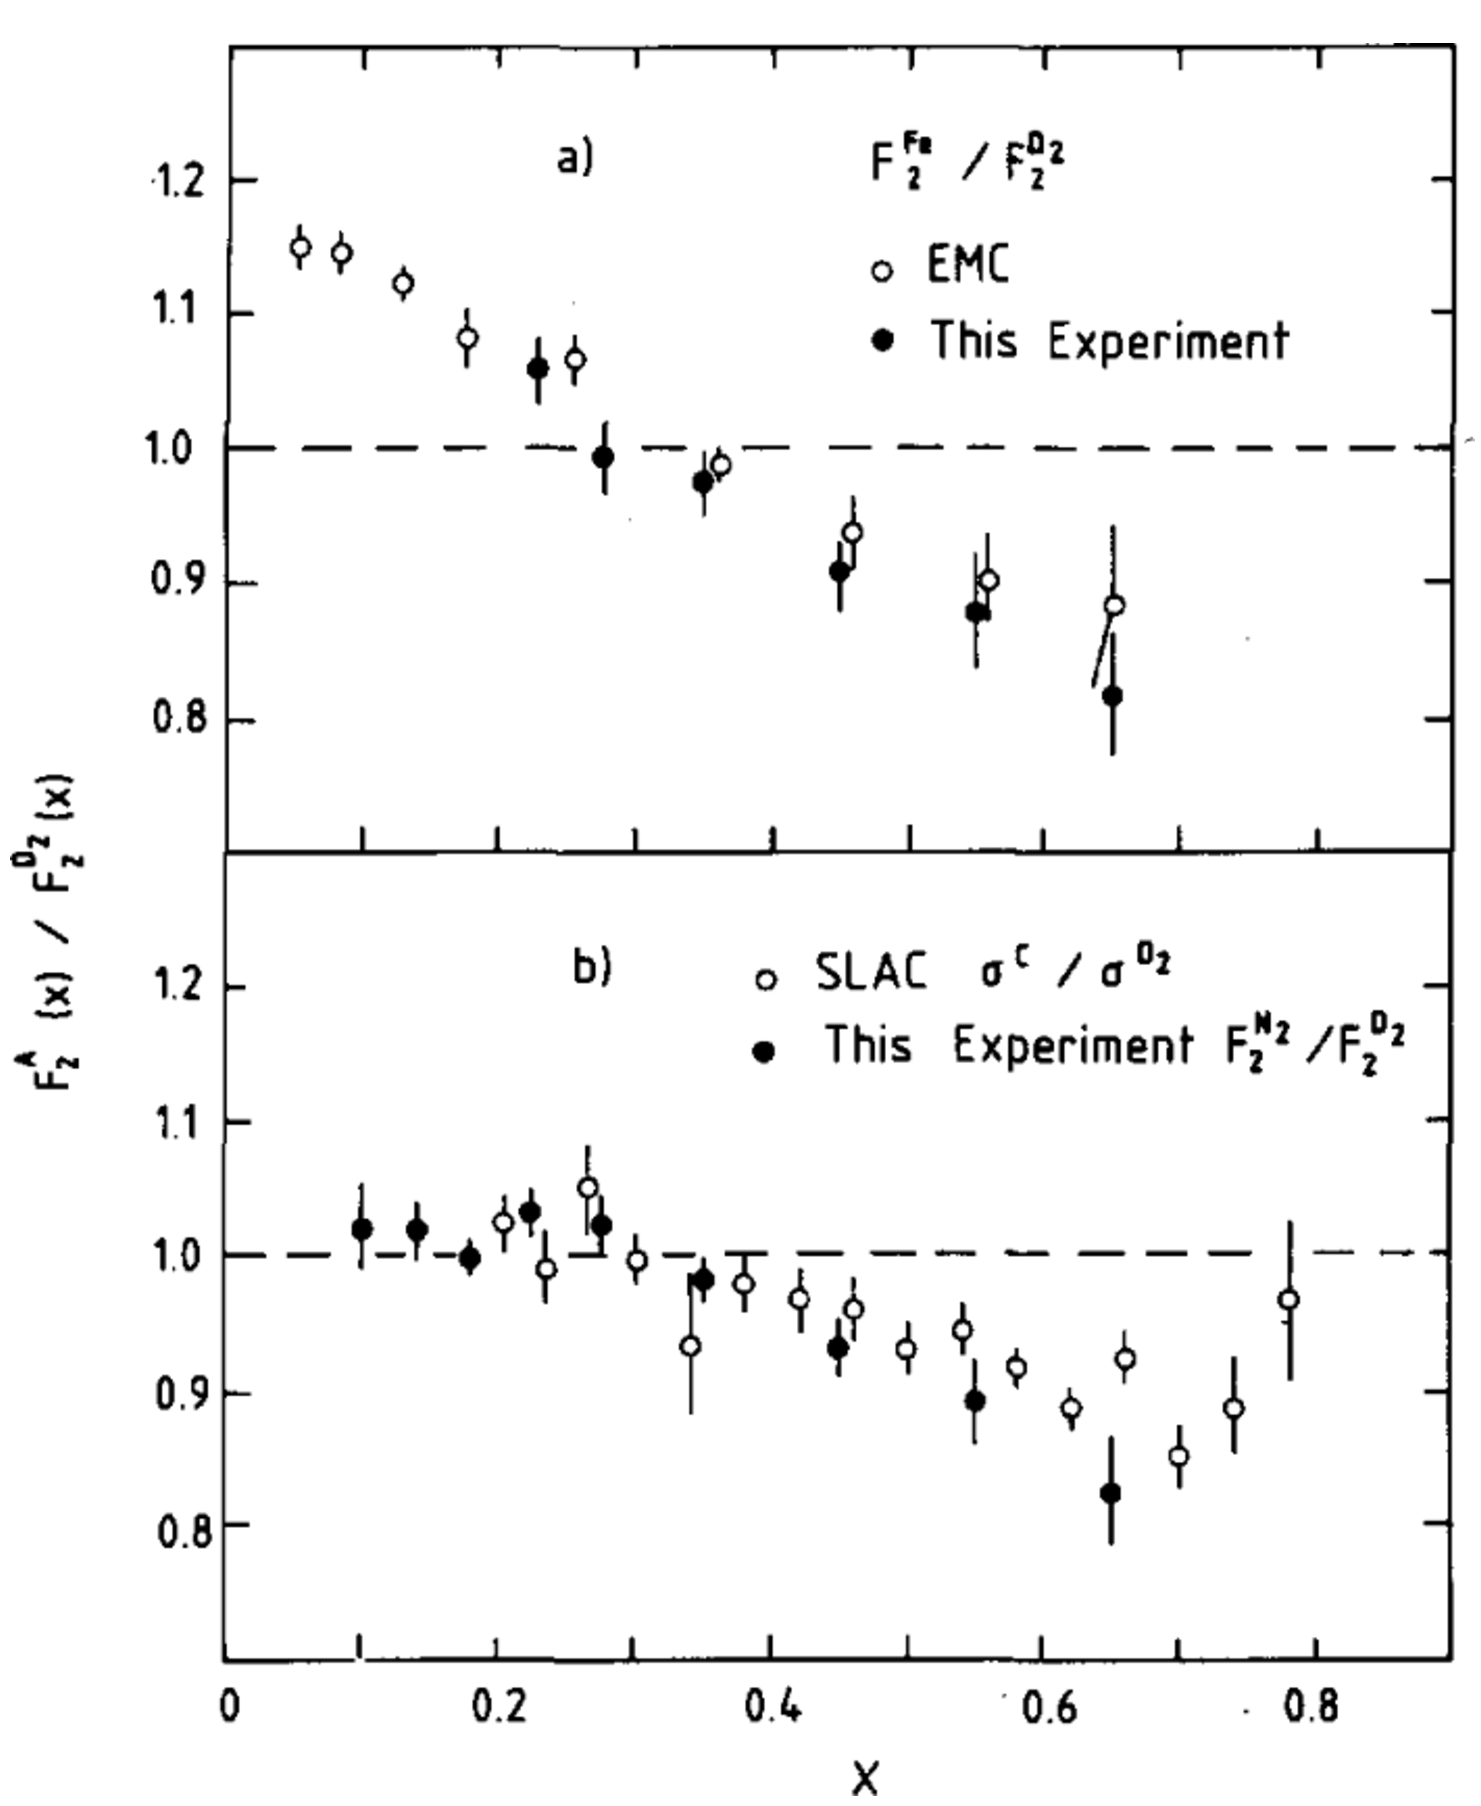
\includegraphics[width=11.0cm]{BCDMS.pdf}
\end{figure}
\paragraph{BCDMS}The Bologna-CERN-Dubna-Munich-Saclay(BCDMS) collaboration at CERN continued the study of the EMC effect by comparing their measurement of the cross section of nitrogen and iron to deuterium. This experiment used a 40m long iron toroid magnet with 8 modules consisting of scintillators and multiwire proportional chambers \cite{BCDMS}. The data collect from this spectrometer is shown in figure \ref{fig:BCDMS}. The BCDMS collaboration compares their data to the EMC collaboration, demonstrating the consistency of their measurement for the EMC effect for iron \cite{BCDMS,Norton}.

\begin{figure}[H]
	\centering
	\caption{The $Q^2$ dependence of ($F_2^n/F_2^p$) for a value of $x$ \cite{ref:NMC}.}
	\label{fig:nmcnp}
	\centering
	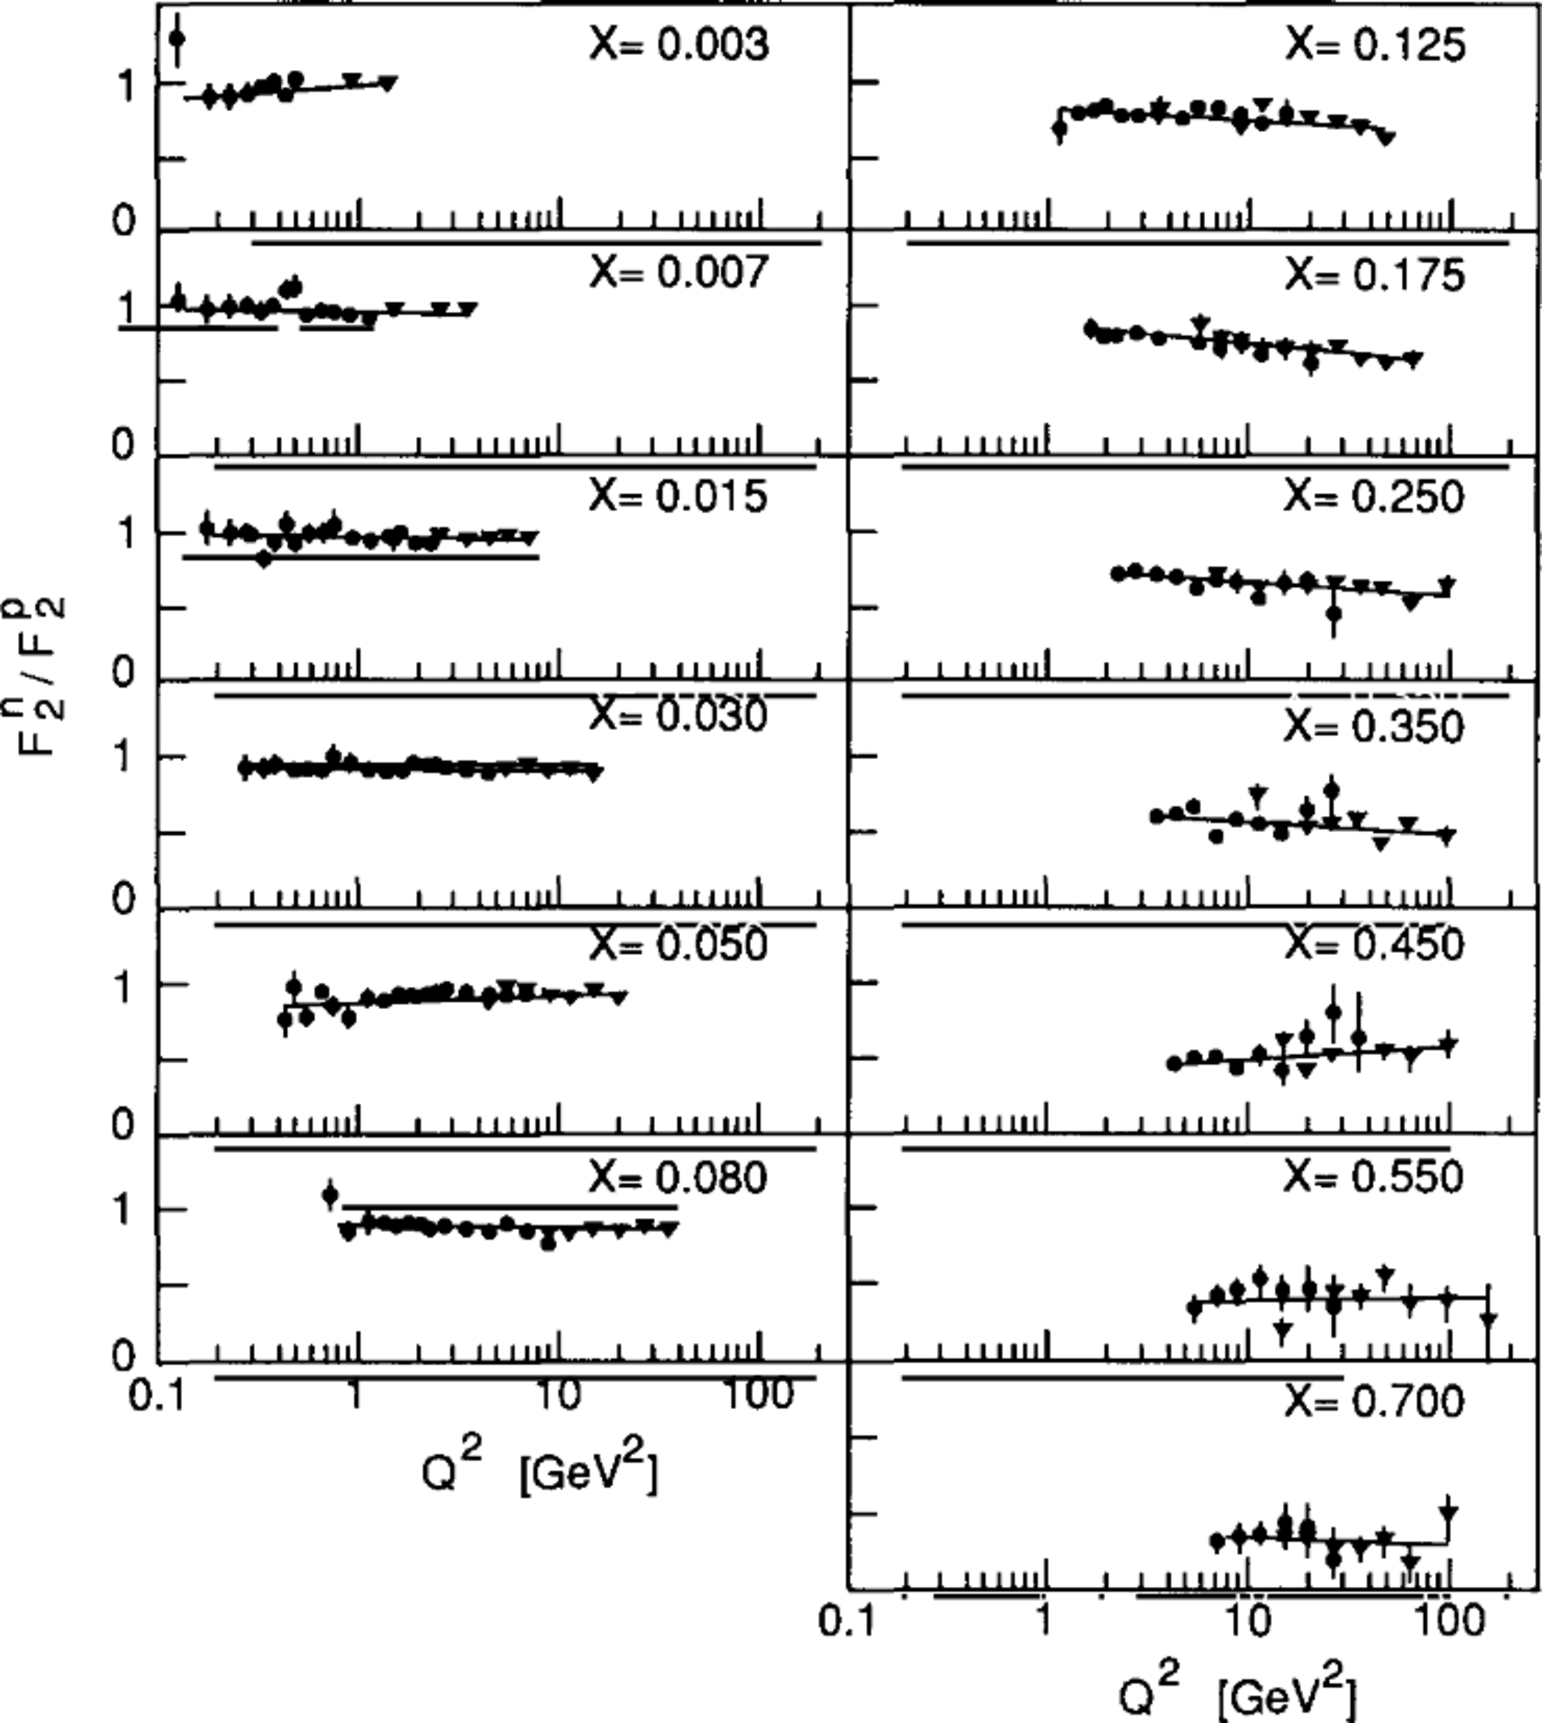
\includegraphics[width=11.75cm]{nmcnp.pdf}
\end{figure}
\paragraph{NMC}In the winter of 1985 the New Muon Collaboration(NMC) purposed to used the muon beam at CERN to expand the understanding of the A dependence for the EMC ratios at low-$x$ and to understand the $Q^2$ dependence of the EMC ratios. Along with the EMC ratios, the NMC also wanted to improve the current measurements for the neutron structure function, $F_2^n$, and the neutron to proton structure function ratio, ($F_2^n/F_2^p$) \cite{NMCtech}. This experiment consisted of completing muon scattering on solid targets of Be, C, Al, Ca, Fe, Sn, and Pb. The data for this experiment covered a kinematic range in $x$ of 0.01 to 0.8, and in $Q^2$ from 2 to 70 GeV$^2$ \cite{ref:NMC}. The NMC concluded the $Q^2$ for the EMC ratios is small and the dependence of A for the EMC effect is approximately logarithmic \cite{ref:NMC,Ajth}. 

\subsection{Experiments at SLAC}
\paragraph{}Scientists at the Stanford Linear Accelerator Center(SLAC) extracted EMC ratios for many nuclei including; $^4$He, $^9$Be, $^{12}$C, $^{27}$Al, $^{40}$Ca, $^{56}$Fe, $^{108}$Ag, and $^{197}$Au. This experiment used an electron beam of 8 to 24.5 GeV. The data spanned a large range of $x$, from 0.089 to 0.8, and $Q^2$ , from 2 to 15 GeV$^2$ to extract cross sections ratios. The EMC ratios were extracted by counting the electrons detected by the SLAC 8-GeV/c magnetic focusing spectrometer \cite{gomez}. The EMC ratios for the eight different nuclear targets are shown in figure \ref{gomez_ma}.
\begin{figure}[h]
	\centering
	\caption{EMC ratios from SLAC. The plots shows the $Q^2$ average cross section ratios with isoscaler corrections for different nuclei \cite{gomez}.}
	\label{gomez_ma}
	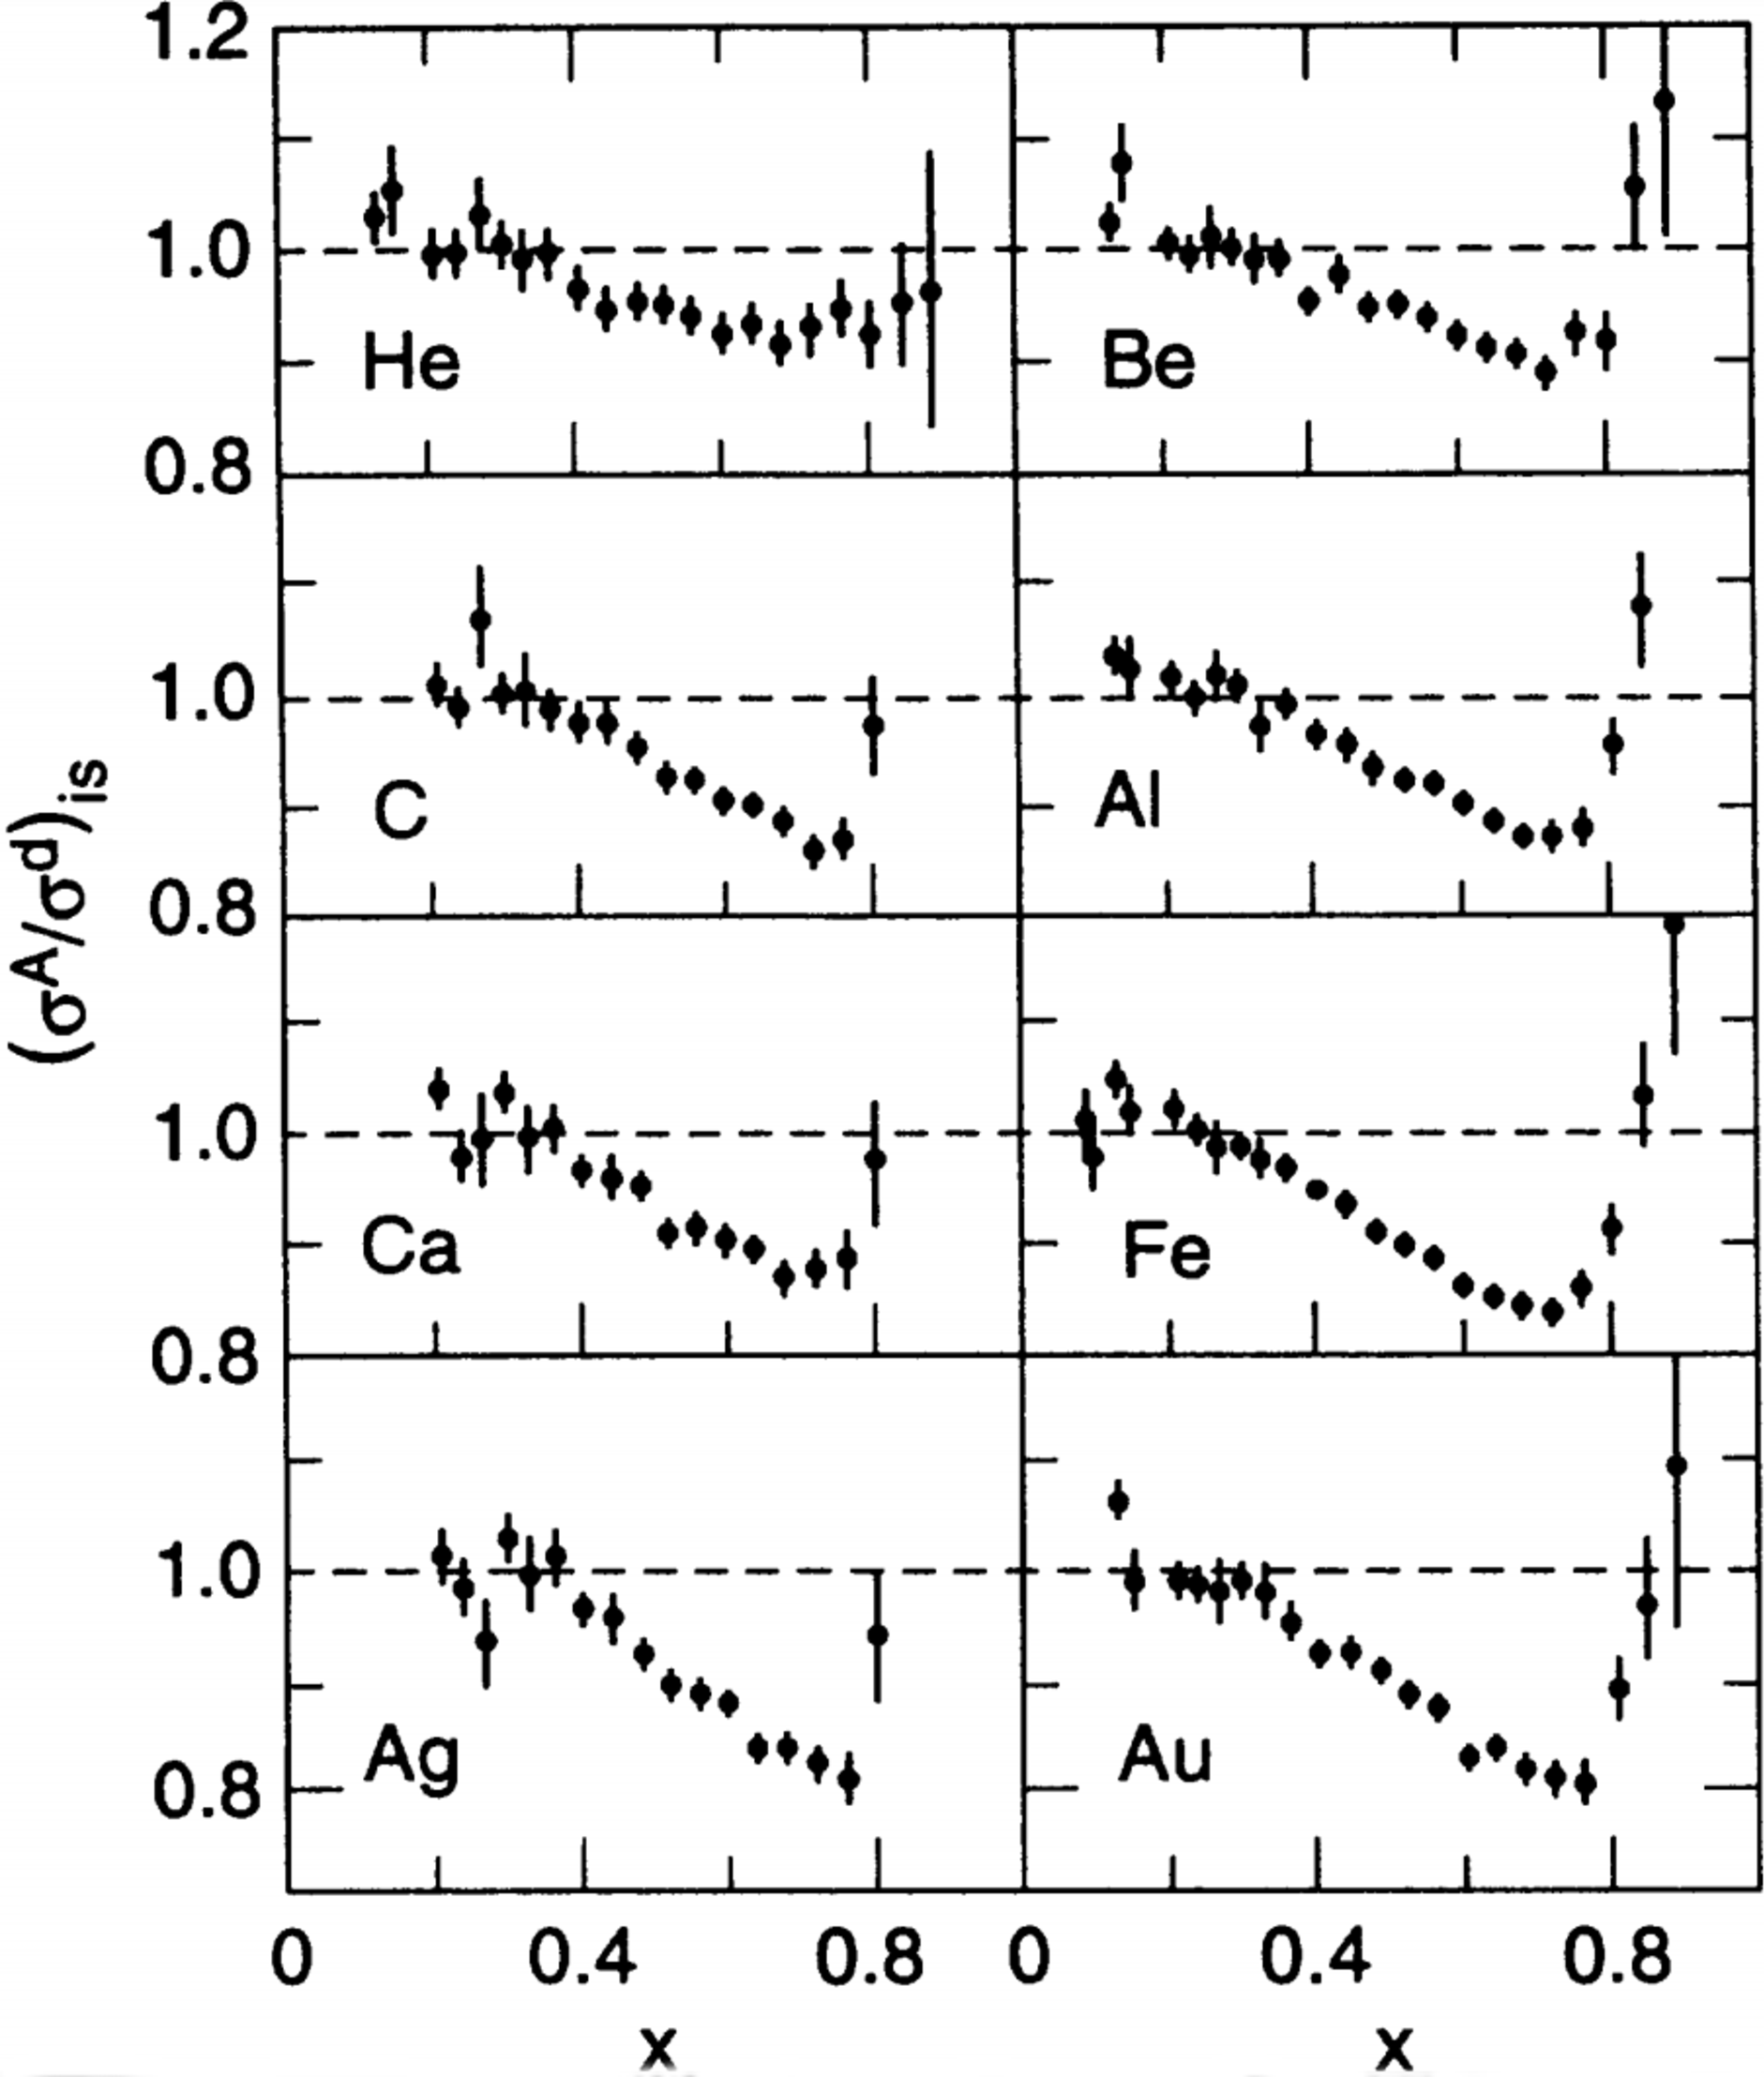
\includegraphics[width=9cm]{slac_ma.pdf} 
\end{figure} 
\paragraph{} The analysis of these ratios revealed the magnitude of the EMC effect, taken to be the A/D ratio at $x=0.6$, was found to be different for the various nuclei, and roughly scaled with the size or density of the nuclei. Figure \ref{gomez_wa}, shows the EMC effect magnitude as a function of the nuclear weight of the targets. It demonstrates an agreement with data from the NMC, that the EMC effect's dependence on A, to be approximately logarithmic \cite{Ajth,gomez,seelyth}. 
\begin{figure}[h]
	\centering
	\caption{The dependence of the atomic mass number on the EMC effect\cite{gomez}.}
	\label{gomez_wa}
	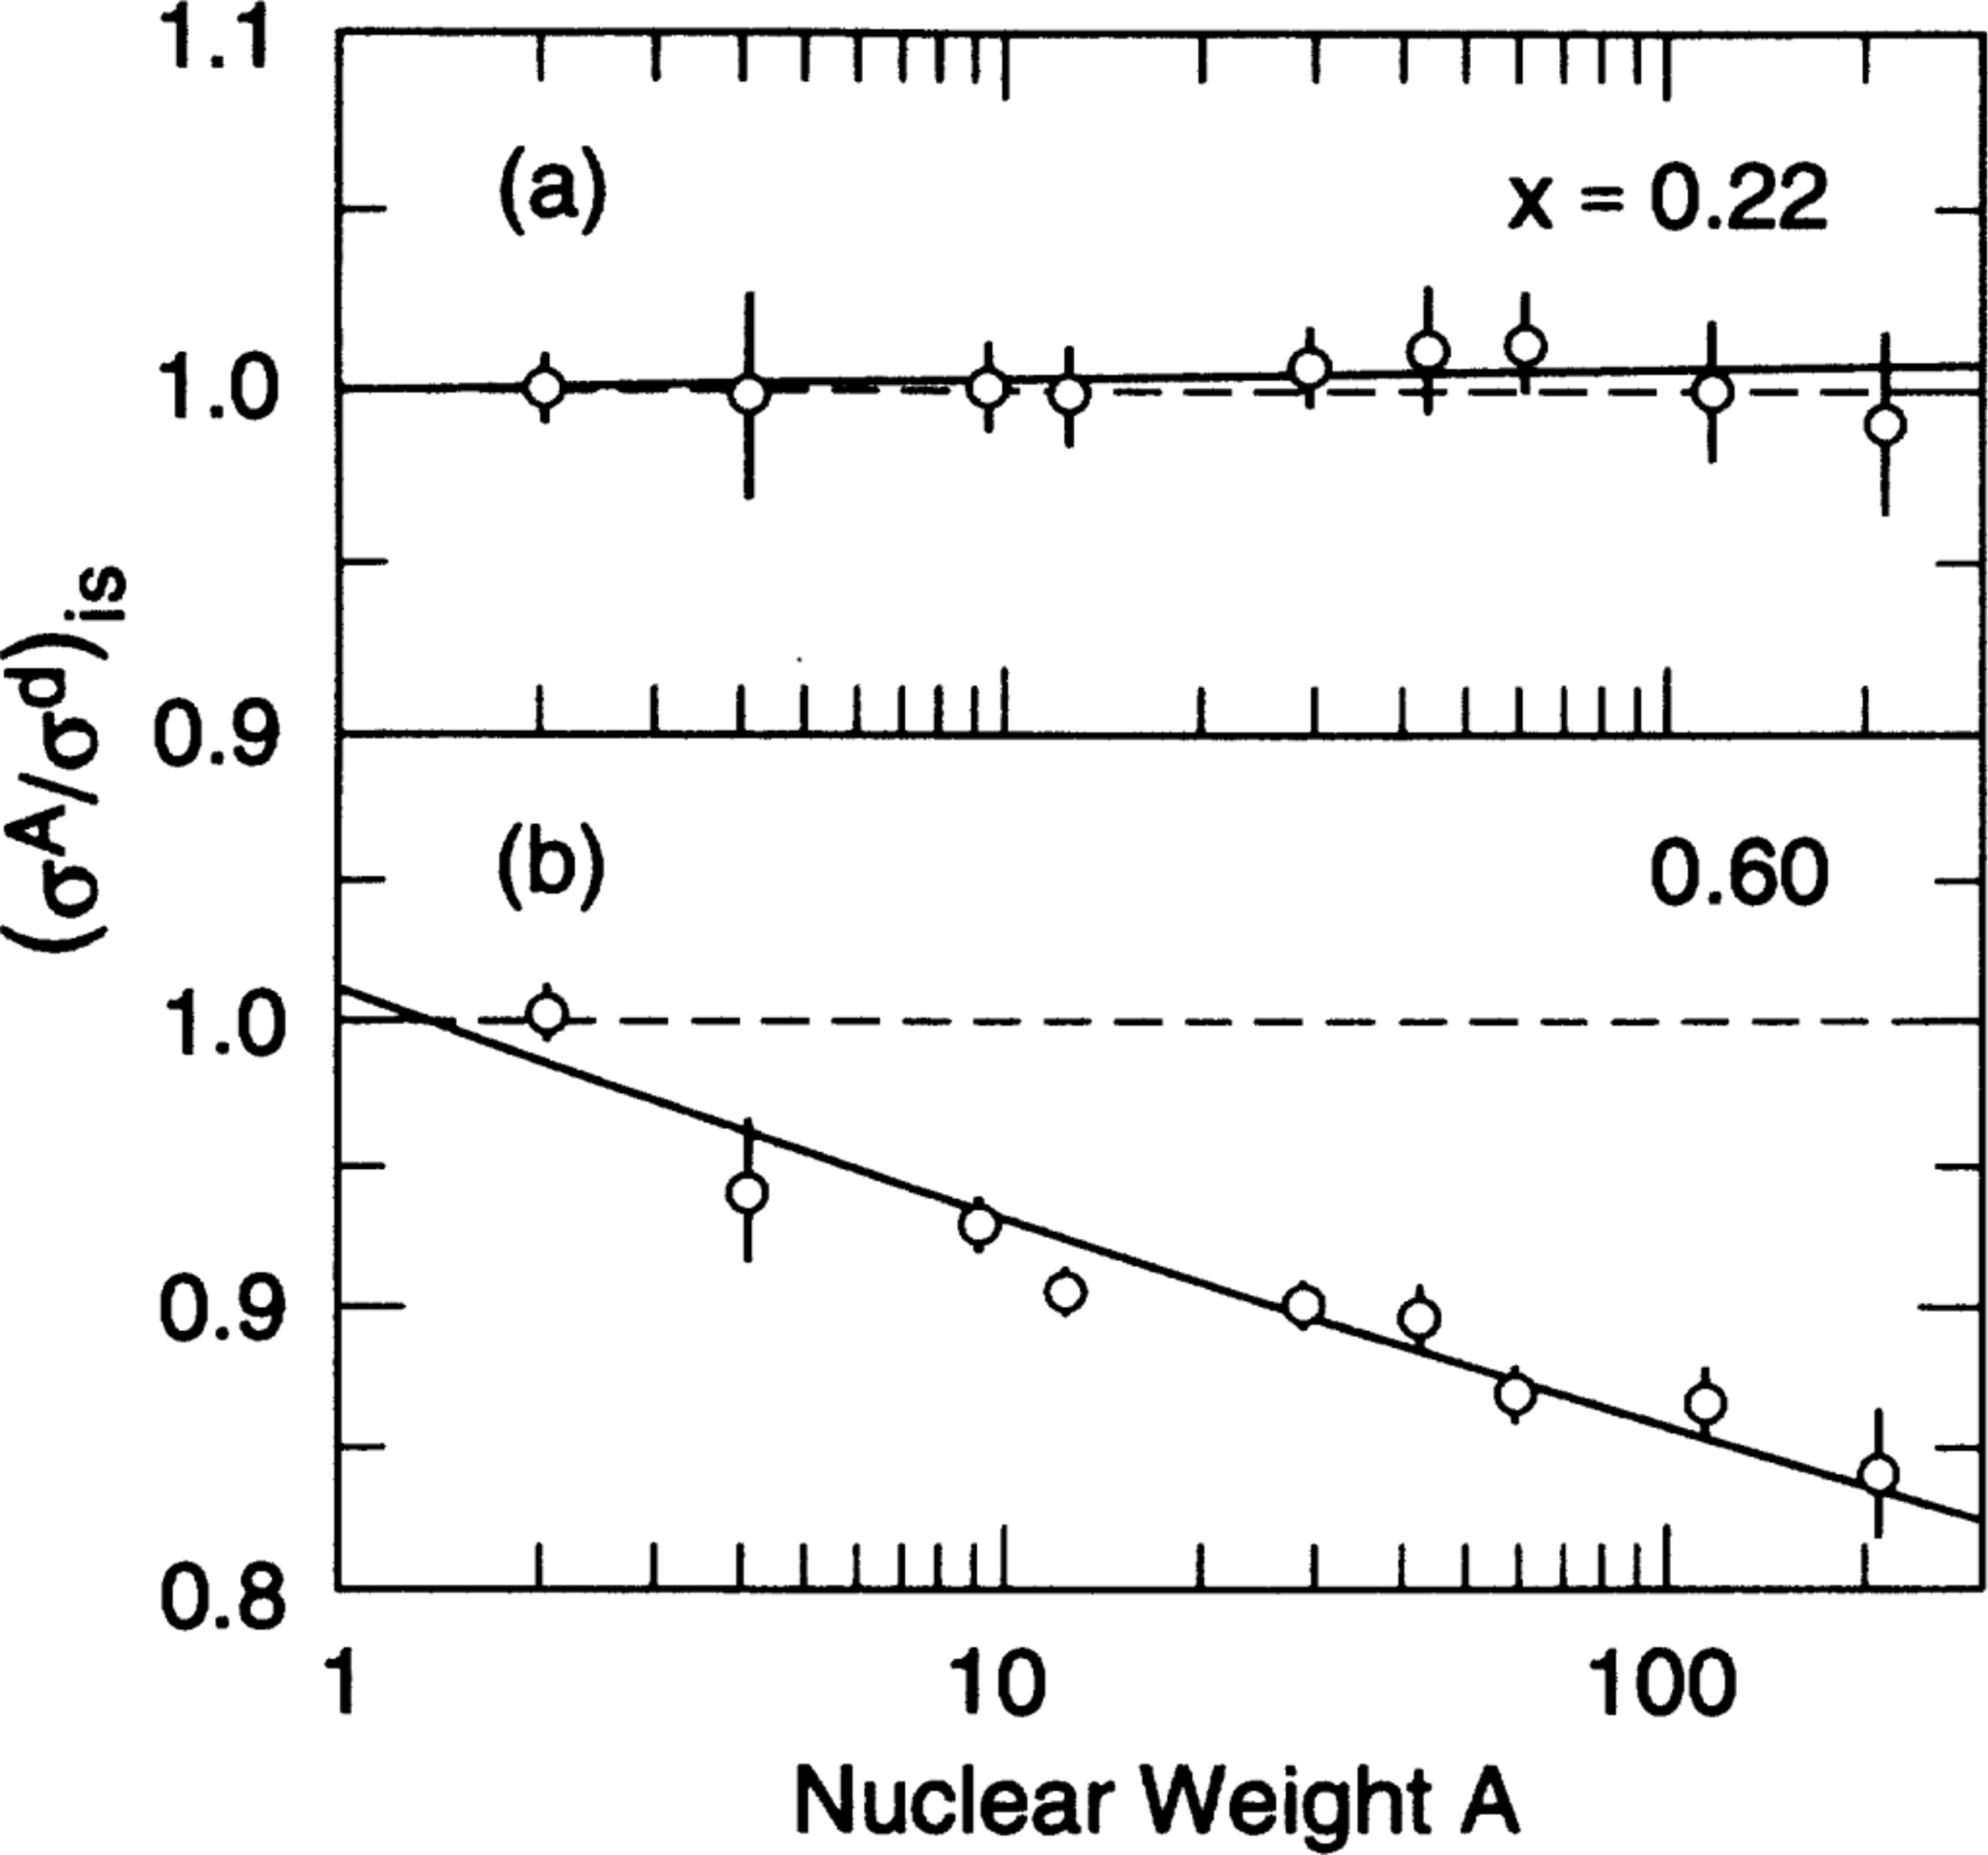
\includegraphics[width=10cm]{slac_wa.pdf} 
\end{figure} 
\subsection{HERMES at DESY}
\paragraph{}
The High-Energy Radiation Megavolt Electron Source(HERMES) collaboration used the Hadron-Electron Ring Accelerator(HERA) at Deutsches Elektronen-Synchrotron (DESY), German Electron Synchrotron, to study the DIS cross section ratios of $^3$He, $^{14}$N, and $^{84}$Kr with respect to D \cite{HERMES_EMC}. Data was collected at $x$ kinematics ranging from 0.010 and 0.65 with $Q^2$ varying between 0.5 and 15 GeV$^2$\cite{HERMES_EMC}. The HERMES collaboration used a 27.5 GeV positron beam to scatter off of gaseous targets into the HERMES forward angle spectrometer. 
\subsection{Experiments at Jefferson Lab}
\paragraph{}Experiments at Thomas Jefferson National accelerator facility(JLab) produced two notable EMC ratio results. In 2006, an experiment designed to study the scaling og the structure function of the target nucleus produced data for the extraction of EMC ratios for C, Fe, and Au. The kinematics of this experiment produced data in the resonance region with a $Q^2 \approx$ 4 $GeV^2/c^2$ and 1.2 $ < W^2 < $ 3 $GeV^2/c^2$. This data is shown in figure \ref{fig:EMCJA} compared with data from SLAC and BCDMS. 
\begin{figure}[H]
	\centering
	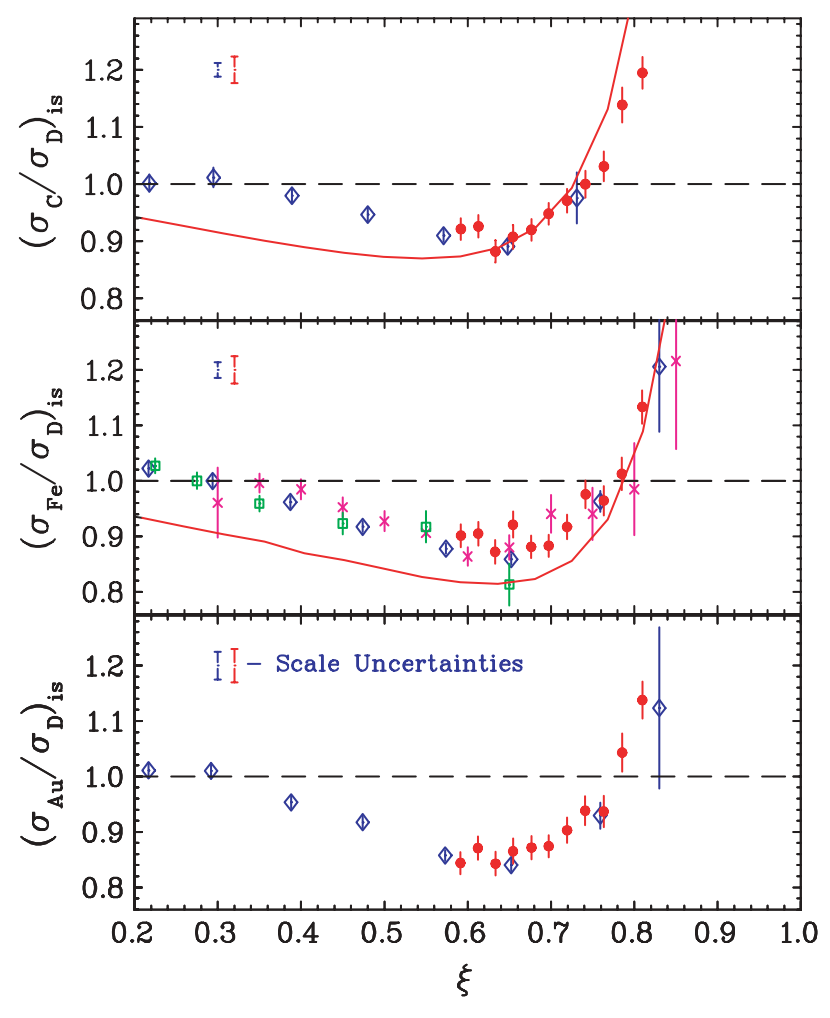
\includegraphics[width=8cm]{EMC_JA.png} 
	\caption{Ratio of nuclear to deuterium cross section per nucleon corrected for neutron excess\cite{EMC_JA}. The JLab data in red is compared with SLAC data in Blue \cite{gomez} and BCDMS data in green \cite{BCDMS}.}
	\label{fig:EMCJA}
\end{figure} 
\begin{equation}
\xi = \frac{2x}{\sqrt{1 + \frac{4M^2x^2}{Q^2}}} \label{xi}
\end{equation}

The SLAC and BCDMS experiments took data in the DIS region with a $W^2 > $ 3 $GeV^2/c^2$. The $Q^2$ value of the data needs to be account for a comparison to made between these three experiments. This has been done by using Nachtmann variable $\xi$, defined in equation \ref{xi} \cite{EMC_JA}. The results show that the EMC ratio in the resonance region matches the same ratio from the DIS region and therefor DIS structure functions information can be extracted from the resonance region \cite{seelyth}. 
\paragraph{}In 2009, results from another Jefferson lab experiment were published describing the EMC effect in very light nuclei. This experiment measured the inclusive cross section from D, $^3$He, $^4$He, $^9$Be, and $^{12}$C for $x$ between 0.3 and 0.9, with $Q^2 \approx$ 3-6 $GeV^2$ \cite{seeley}.  This experiment provided the first results for $^3$He EMC ratios for high $x$.  Also, results from all of the nuclear targets showed that the nuclear dependence of the EMC effect may depend on the local nuclear environment \cite{seeley}. Previous results showed a logarithmic dependence of the EMC effect on A. The EMC results for $^9$Be create a disagreement from past results. This analysis is shown in figure \ref{EMCrho} \cite{seeley}.

\iffalse
\begin{figure}[h]
	\centering
	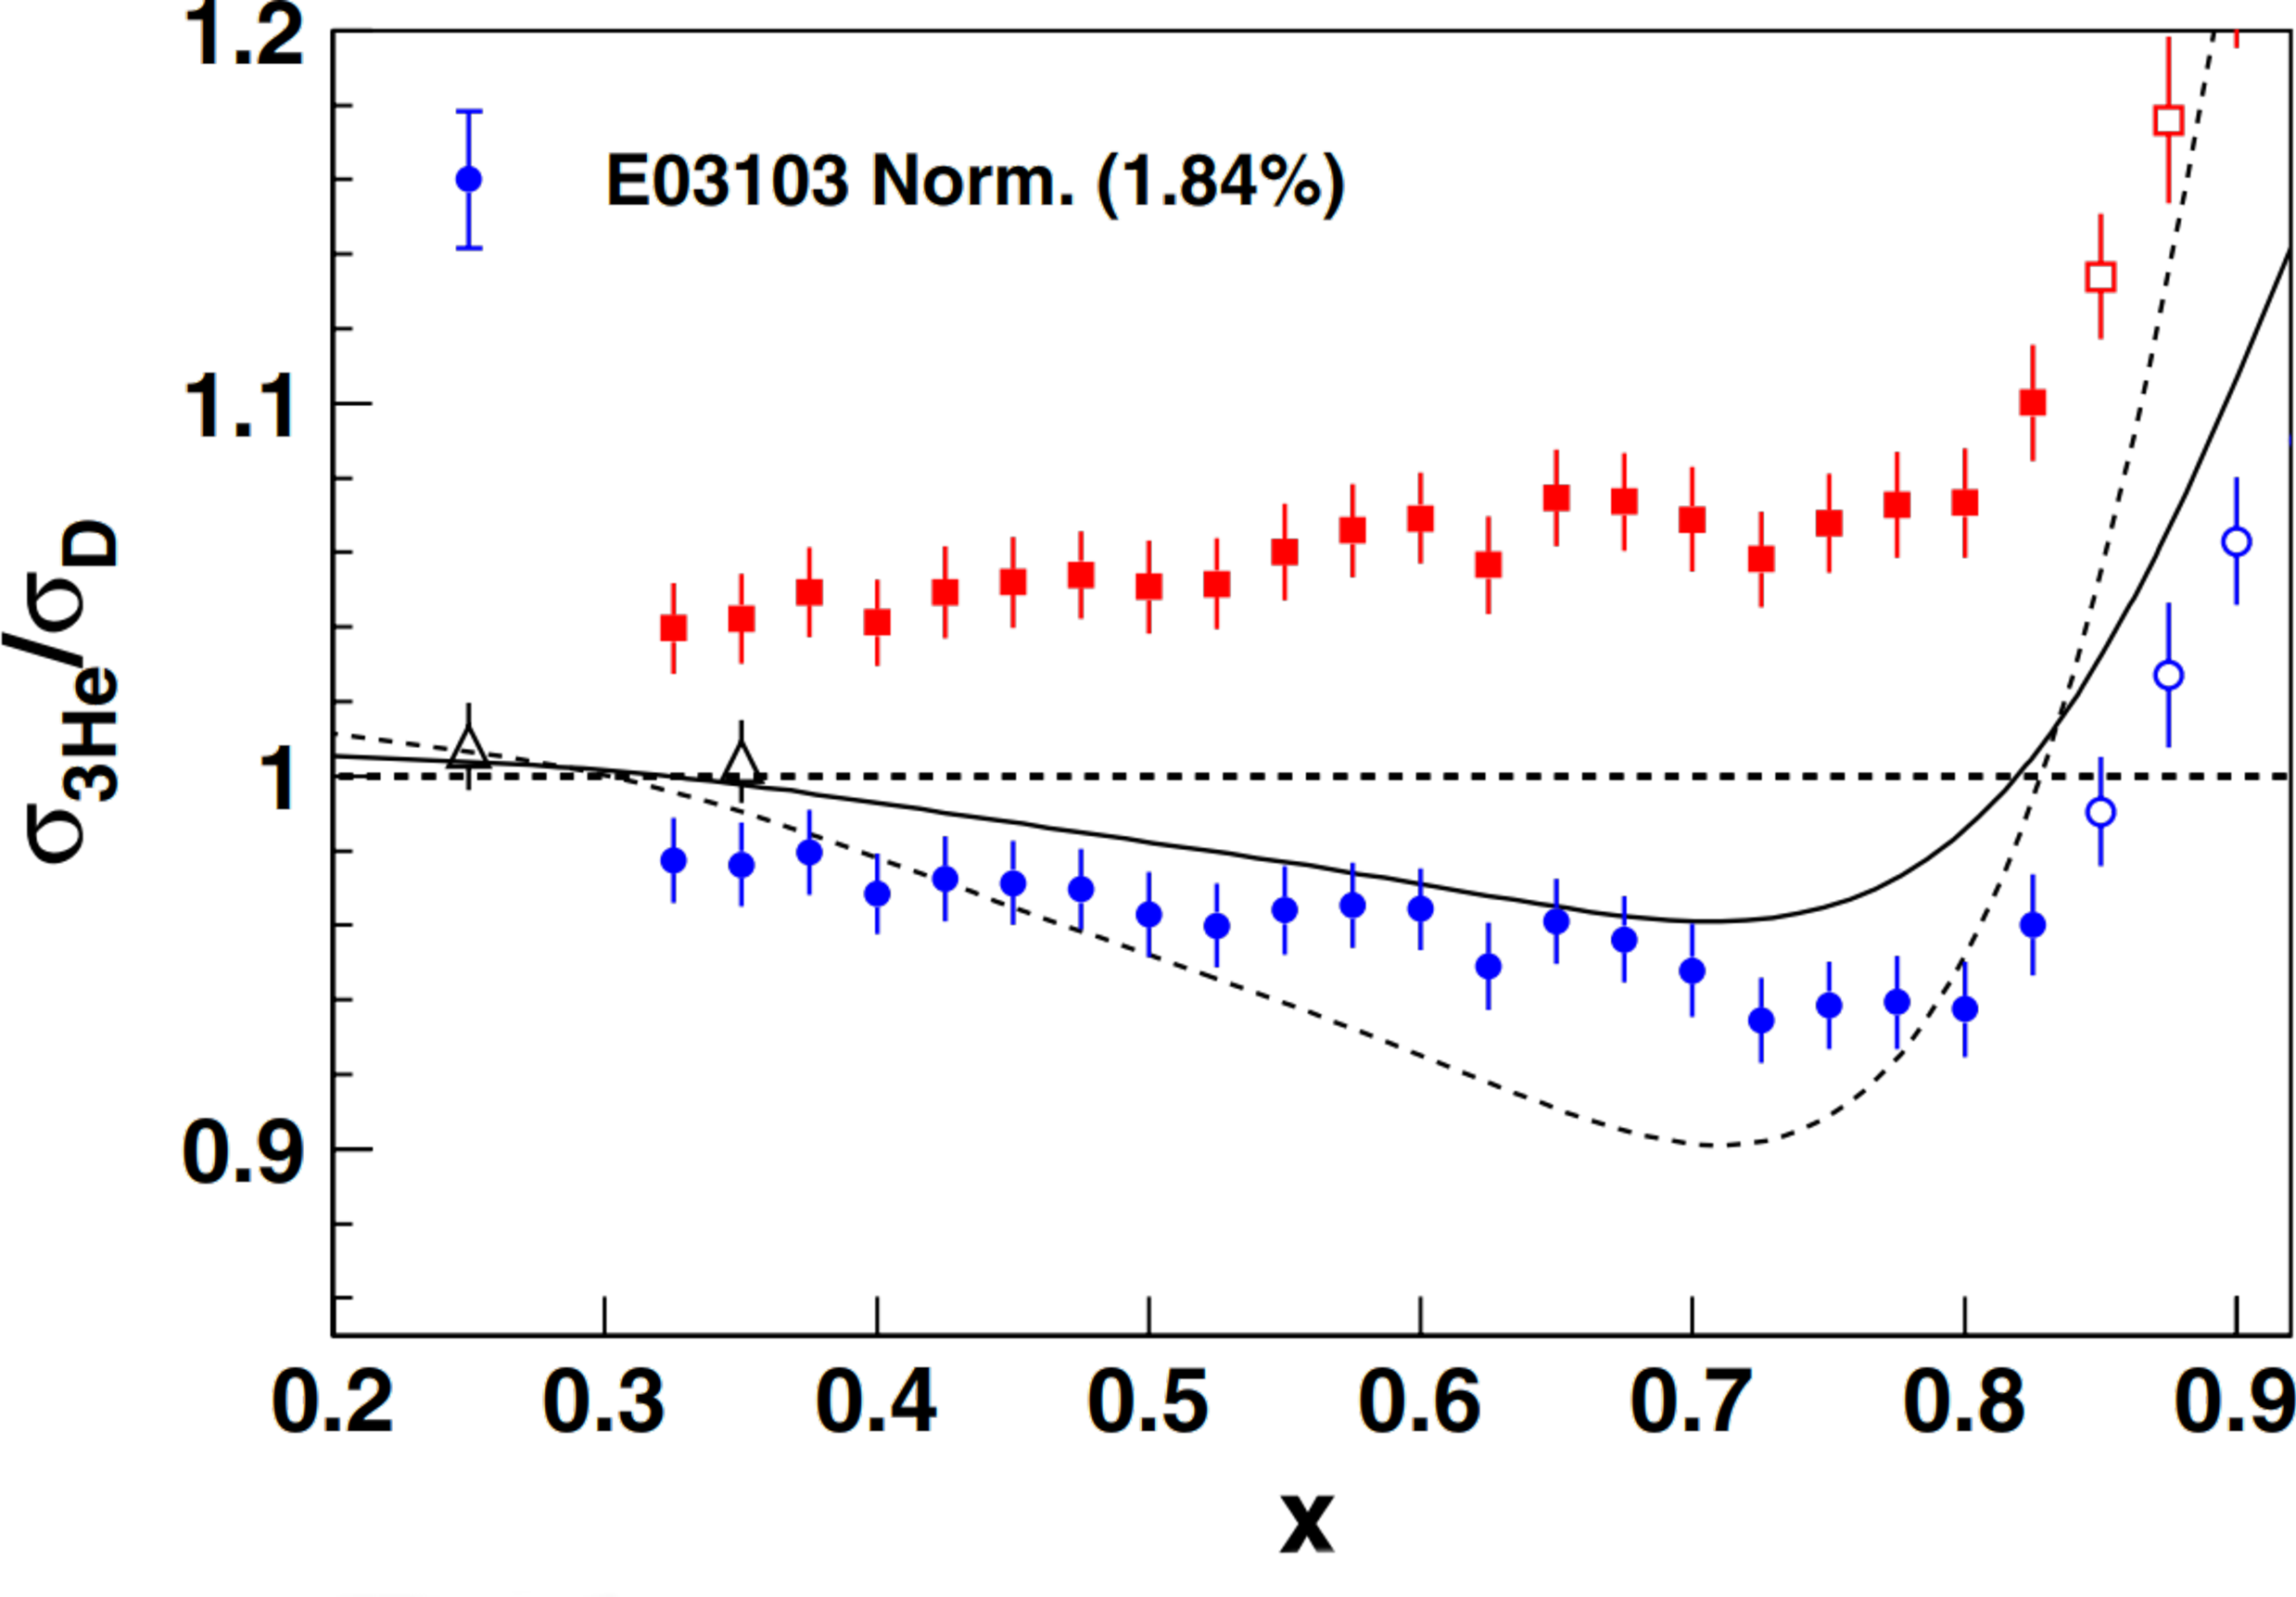
\includegraphics[width=10cm]{He3_EMC_seely.pdf} 
	\caption{EMC ratio for He3, Blue points are corrected for proton excess\cite{seeley}.}
	\label{EMCHe3_Seely}
\end{figure} 
\fi

\begin{figure}[h]
	\centering
	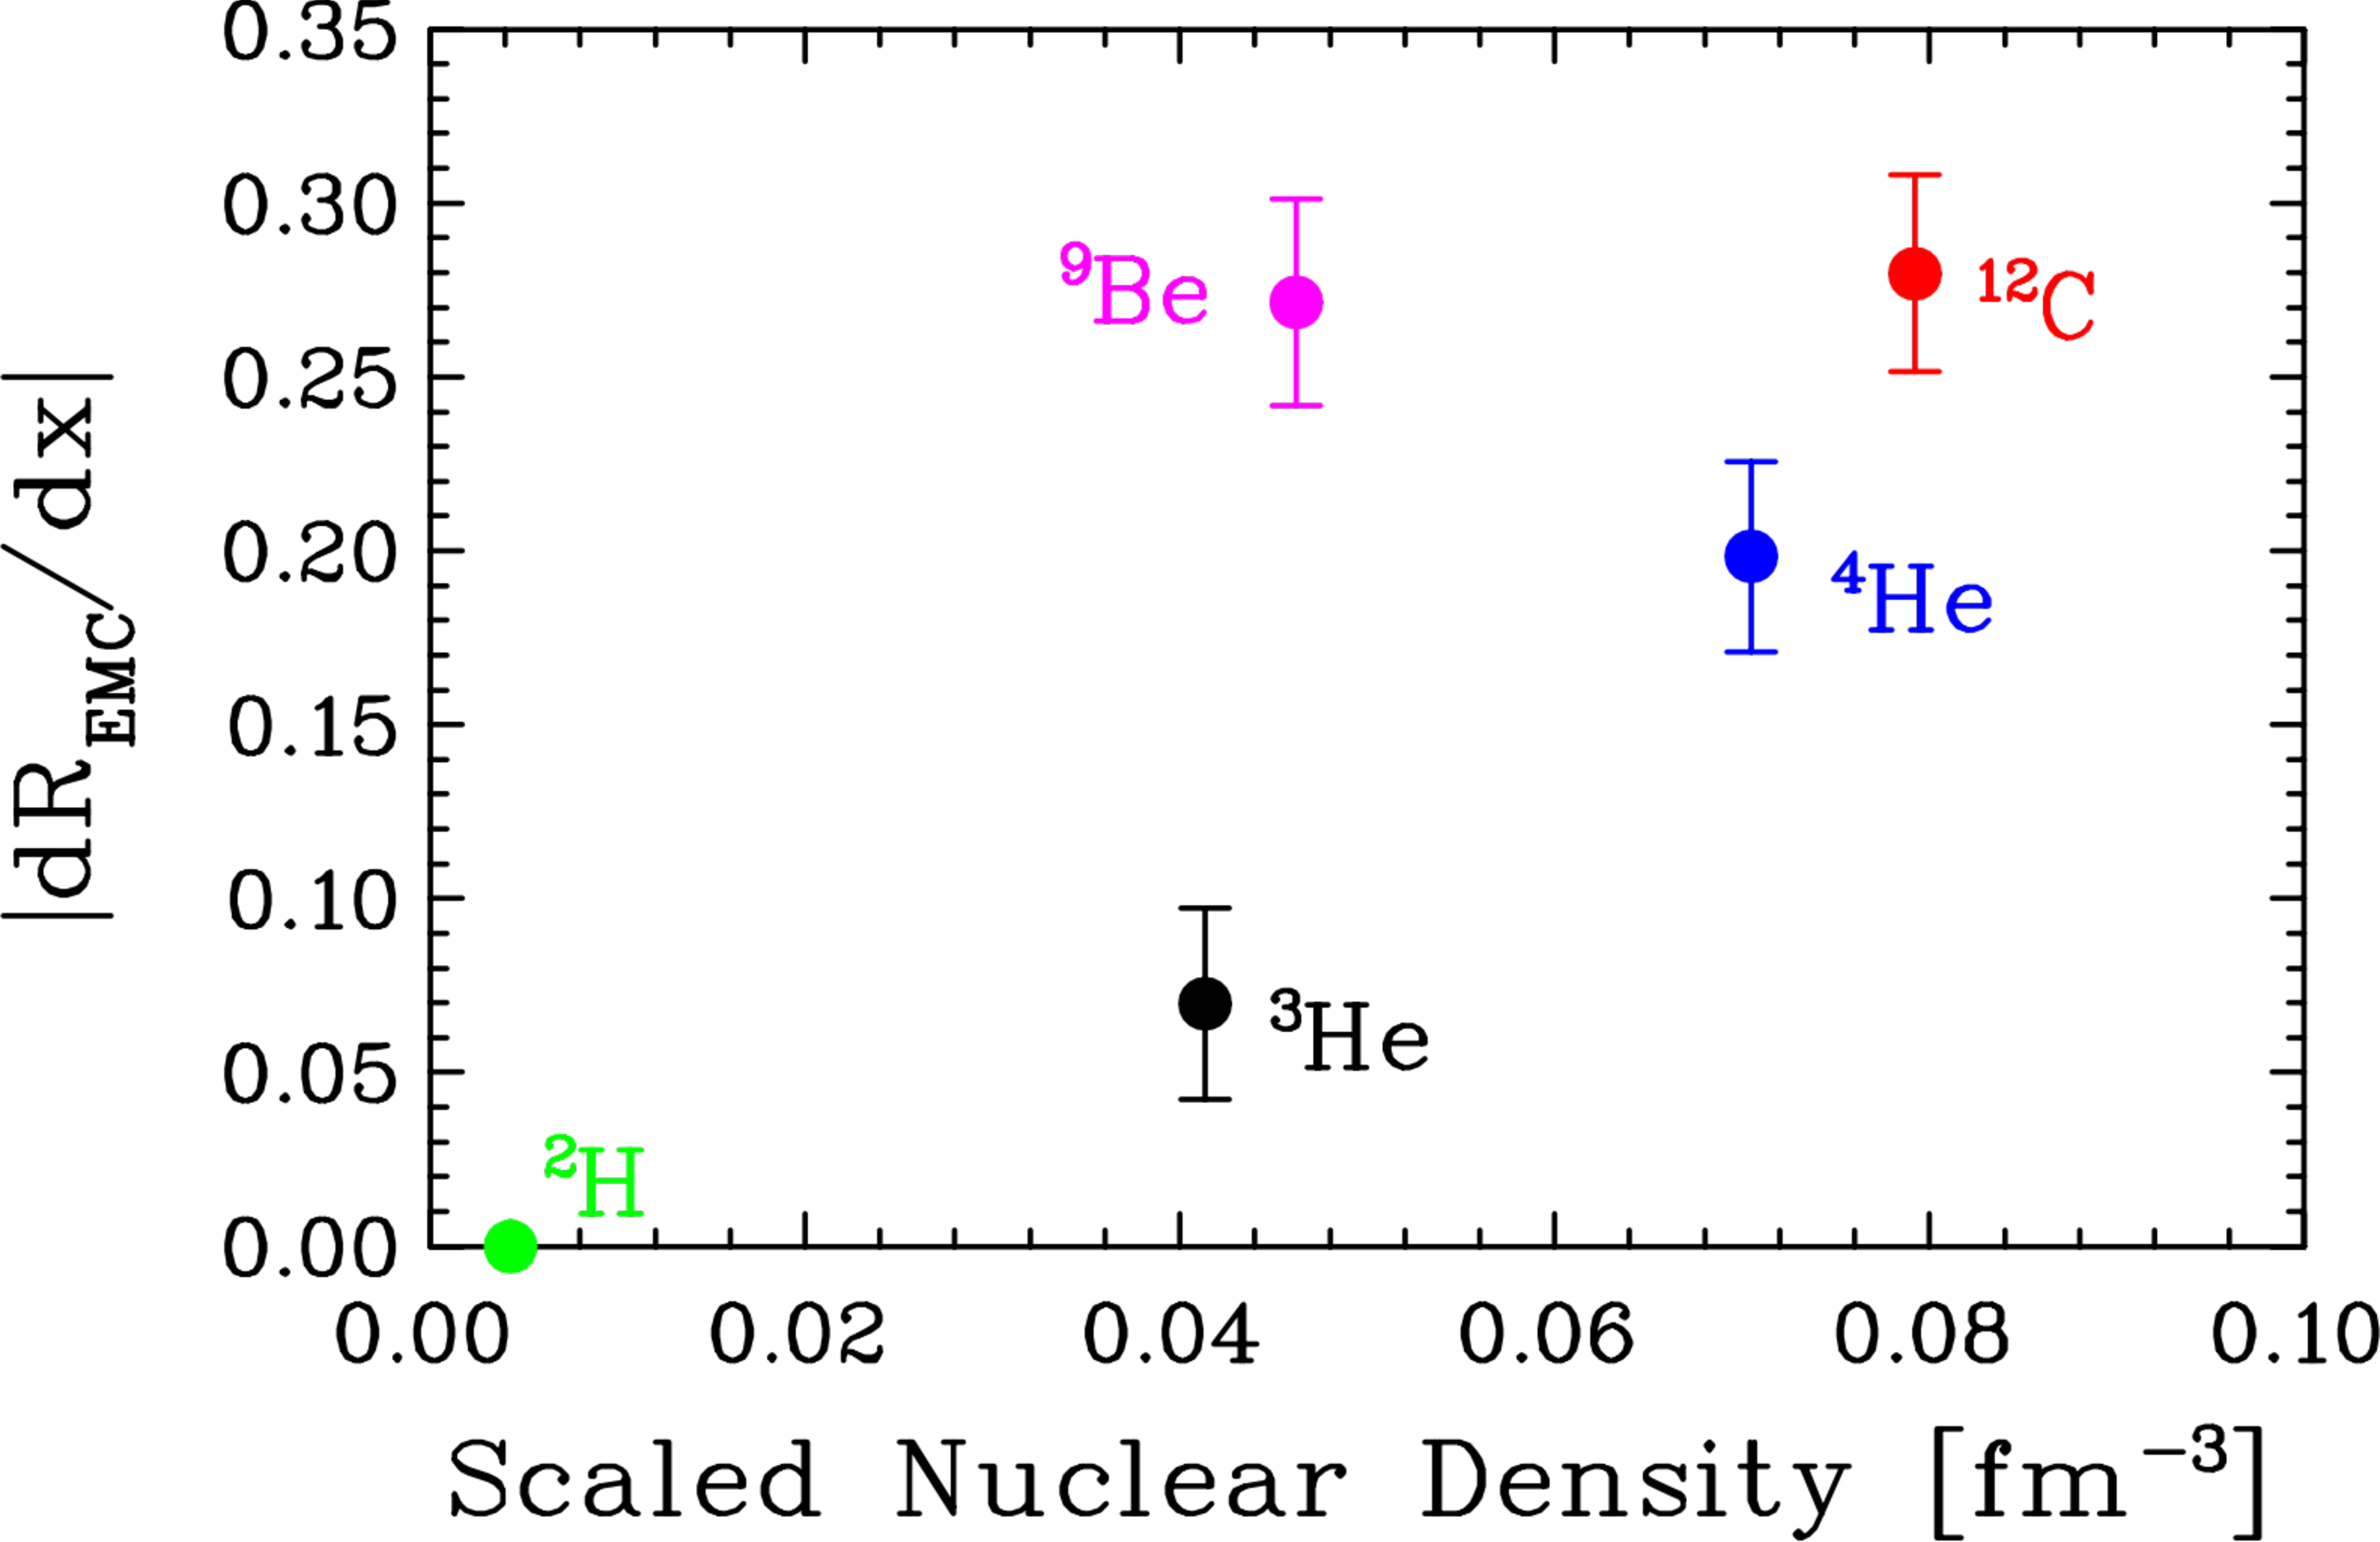
\includegraphics[width=10cm]{EMC_rho.pdf} 
	\caption{Isoscalar EMC effect as function of nuclear density \cite{seeley}.}
	\label{EMCrho}
\end{figure} 

\section{EMC Theory and Models}
\paragraph{}Since the founding of the EMC effect, there has been numerous amounts of work conducted on the theories to describe these EMC ratios. The models attempt to characterize both the nuclear and nucleon structure functions for the entire range of $x$ from 0.0 to 1.0. This section will briefly discuss the basic idea of a few EMC models.
\subsection{Multiquark Cluster}
\paragraph{} The multiquark cluster model discussed by K. M. Hanna et. al. \cite{EMC_multiQ} and R. L. jaffe \cite{EMC_multiQ_2} , states that it is possible to form color singlet quark clusters inside of a dense nucleus. These quark clusters can contain 3N quarks (3,6,9...) \cite{Norton}. These quark clusters have the possibility to contain the momentum of multiple nucleons \cite{Ajth}. Because of the overall momentum of these clusters, the multiquark cluster models makes predictions for high $x $, but these clusters are not understood enough to make predictions at low $x$ \cite{Geesaman, EMC_model_1, EMC_multiQ, Ajth}.  

\subsection{Nuclear Binding}
\paragraph{} Describing the EMC effect via nuclear binding was first attempted by Akulinechev et. al. \cite{EMC_binding_3} and Dunne and Thomas \cite{EMC_binding_2}. For the nuclear binding model, an average nucleon has a momentum and a separation energy defined as $\vec{p}$ and $\langle \epsilon \rangle$ respectively \cite{Norton}. The inclusion of the separation energy in the definition of momentum of the post scattering A-1 system causes a manipulation in the value of $x$. $x$ becomes $x^{\prime} = \frac{Q^2}{2p^{\prime}\cdot q}$, where $p^{\prime}$ is (M + $\epsilon$, $\vec{p}$) \cite{Norton}. The modification of the momentum through nuclear binding allows this EMC model to explain the EMC effect and the sharp rise in the fermi motion area, but fails to correctly describe the rise in the anti-shawdowing region around $x$ = 0.2 \cite{EMC_binding, EMC_model_1, Ajth}.

\subsection{Medium Modification}
\paragraph{} Smith and Miller \cite{EMC_medium_2} claim that measurements of nuclear observable could be explained by modifications of the nuclear structure due to the medium. The medium is filled with external fields created by the surrounding nucleons. These fields modify the quark waveform of a single nucleon. Using medium modifications C. Cloet, W. Bentz, and A. W. Thomas \cite{EMC_medium_1} were able to describe the EMC effect for a collection of nuclear targets and calculate the correct A dependence of the EMC effect. 


\subsection{Rescaling}
\paragraph{} Nachtmann and Pierner \cite{EMC_rescaling_2} and Close et al \cite{EMC_rescaling_1} discovered a way to relate the DIS structure function of Fe and D with scaling variable. They found that by using a relative shift in the scale of the $Q^2$ value that $F_2^{Fe}(Q^2) =F_2^{D}(\xi Q^2)$ \cite{Geesaman}. Both teams proposed that as nuclei get heavier their quarks are bound in an area larger compared to the confinement area for a free nucleon. This dynamic rescaling model is applicable for 0.2 $ < x <$ 0.8, but does not match the EMC ratio for the Fermi motion region with $x > 0.8$ \cite{EMC_model_1, EMC_rescaling_1, Geesaman, EMC_rescaling_2}.

\paragraph{} The models discussed hear are only a small subset of the models that have been used to describe the EMC ratios. The downfall for most of these models is the inability to consistently predict the EMC ratio for all nuclear targets and for the entire range of $x$ in DIS. In order to better constrain the EMC effect and gain a better understanding of DIS, we need to conduct more experiments directly targeting specific regions of the complex problem.  

\chapter{MARATHON}
\paragraph{}Experiment E12-010-102, MARATHON (MeAsurement of the $F_2^n$/$F_2^p$,$d$/$u$ RAtios and A=3 EMC Effect in Deep Inelastic Electron Scattering Off the Tritium and Helium MirrOr Nuclei), will use deep inelastic scattering off of the mirror nuclei $^3$H and $^3$He to measure the EMC effect for both $^3$H and $^3$He, to determine the ratio of the neutron to proton inelastic structure functions, and to find the ratio of the down to up quark distributions in the nucleon \cite{Marathon}.
\paragraph{}The MARATHON experiment will provide DIS data to determine the EMC effect for the two A=3 mirror nuclei. Previous experiments to measure the $^3$He EMC ratios where able to gather data at low and medium $x$ for DIS kinematics, and only data in the resonance region for higher $x$.  


